\subsection{Memcached}
\label{sec:mcd}

\begin{figure*}
\centering
%\vspace*{-0.3cm}  
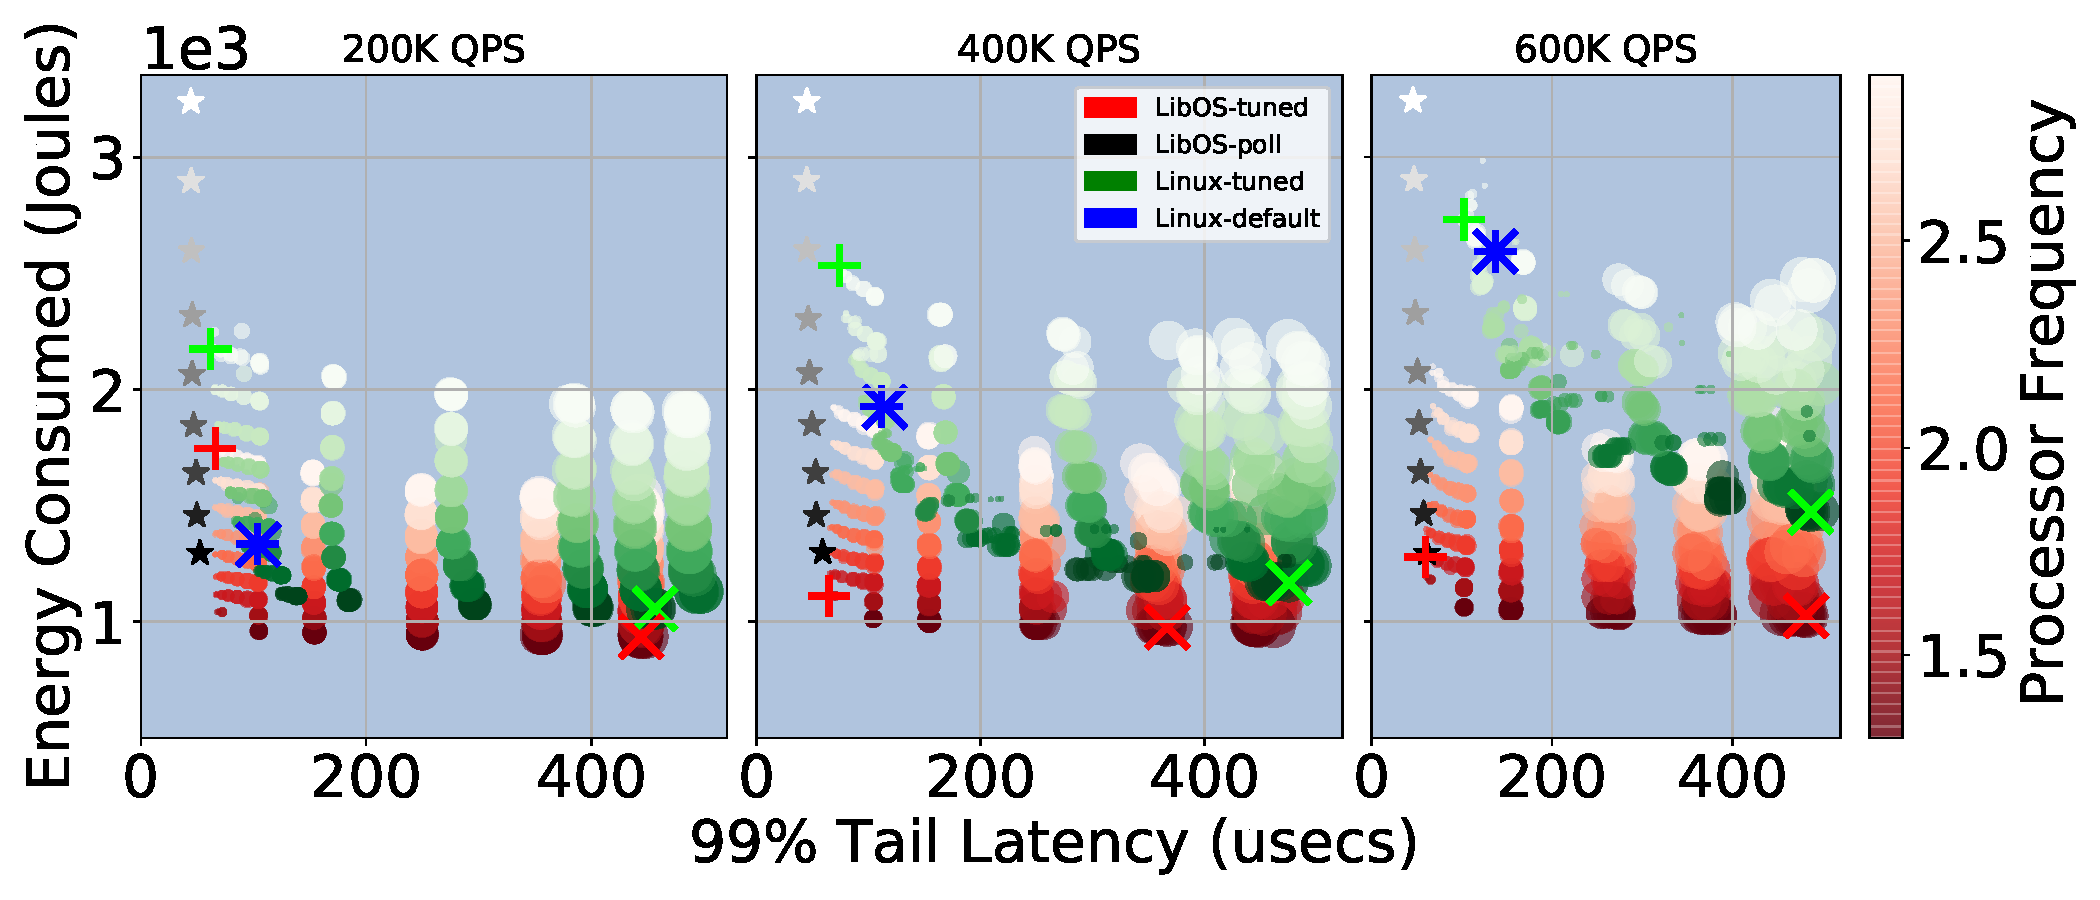
\includegraphics[width=1\textwidth]{figures/mcd_overview}
\caption[]
%{\small 
{Overview of memcached experiments across 200K, 400K, and 600K QPS. Each circle represents an experimental run of tuning ITR-delay and DVFS. The larger the size of a circle equates to larger ITR-delay value. The darkening of color gradient indicates slowing down processor frequency. The \textbf{x} indicate lowest energy consumption. The \textbf{+} indicate lowest tail latency.}
\label{fig:mcd_overview}
\end{figure*}
\begin{figure}
%\centering
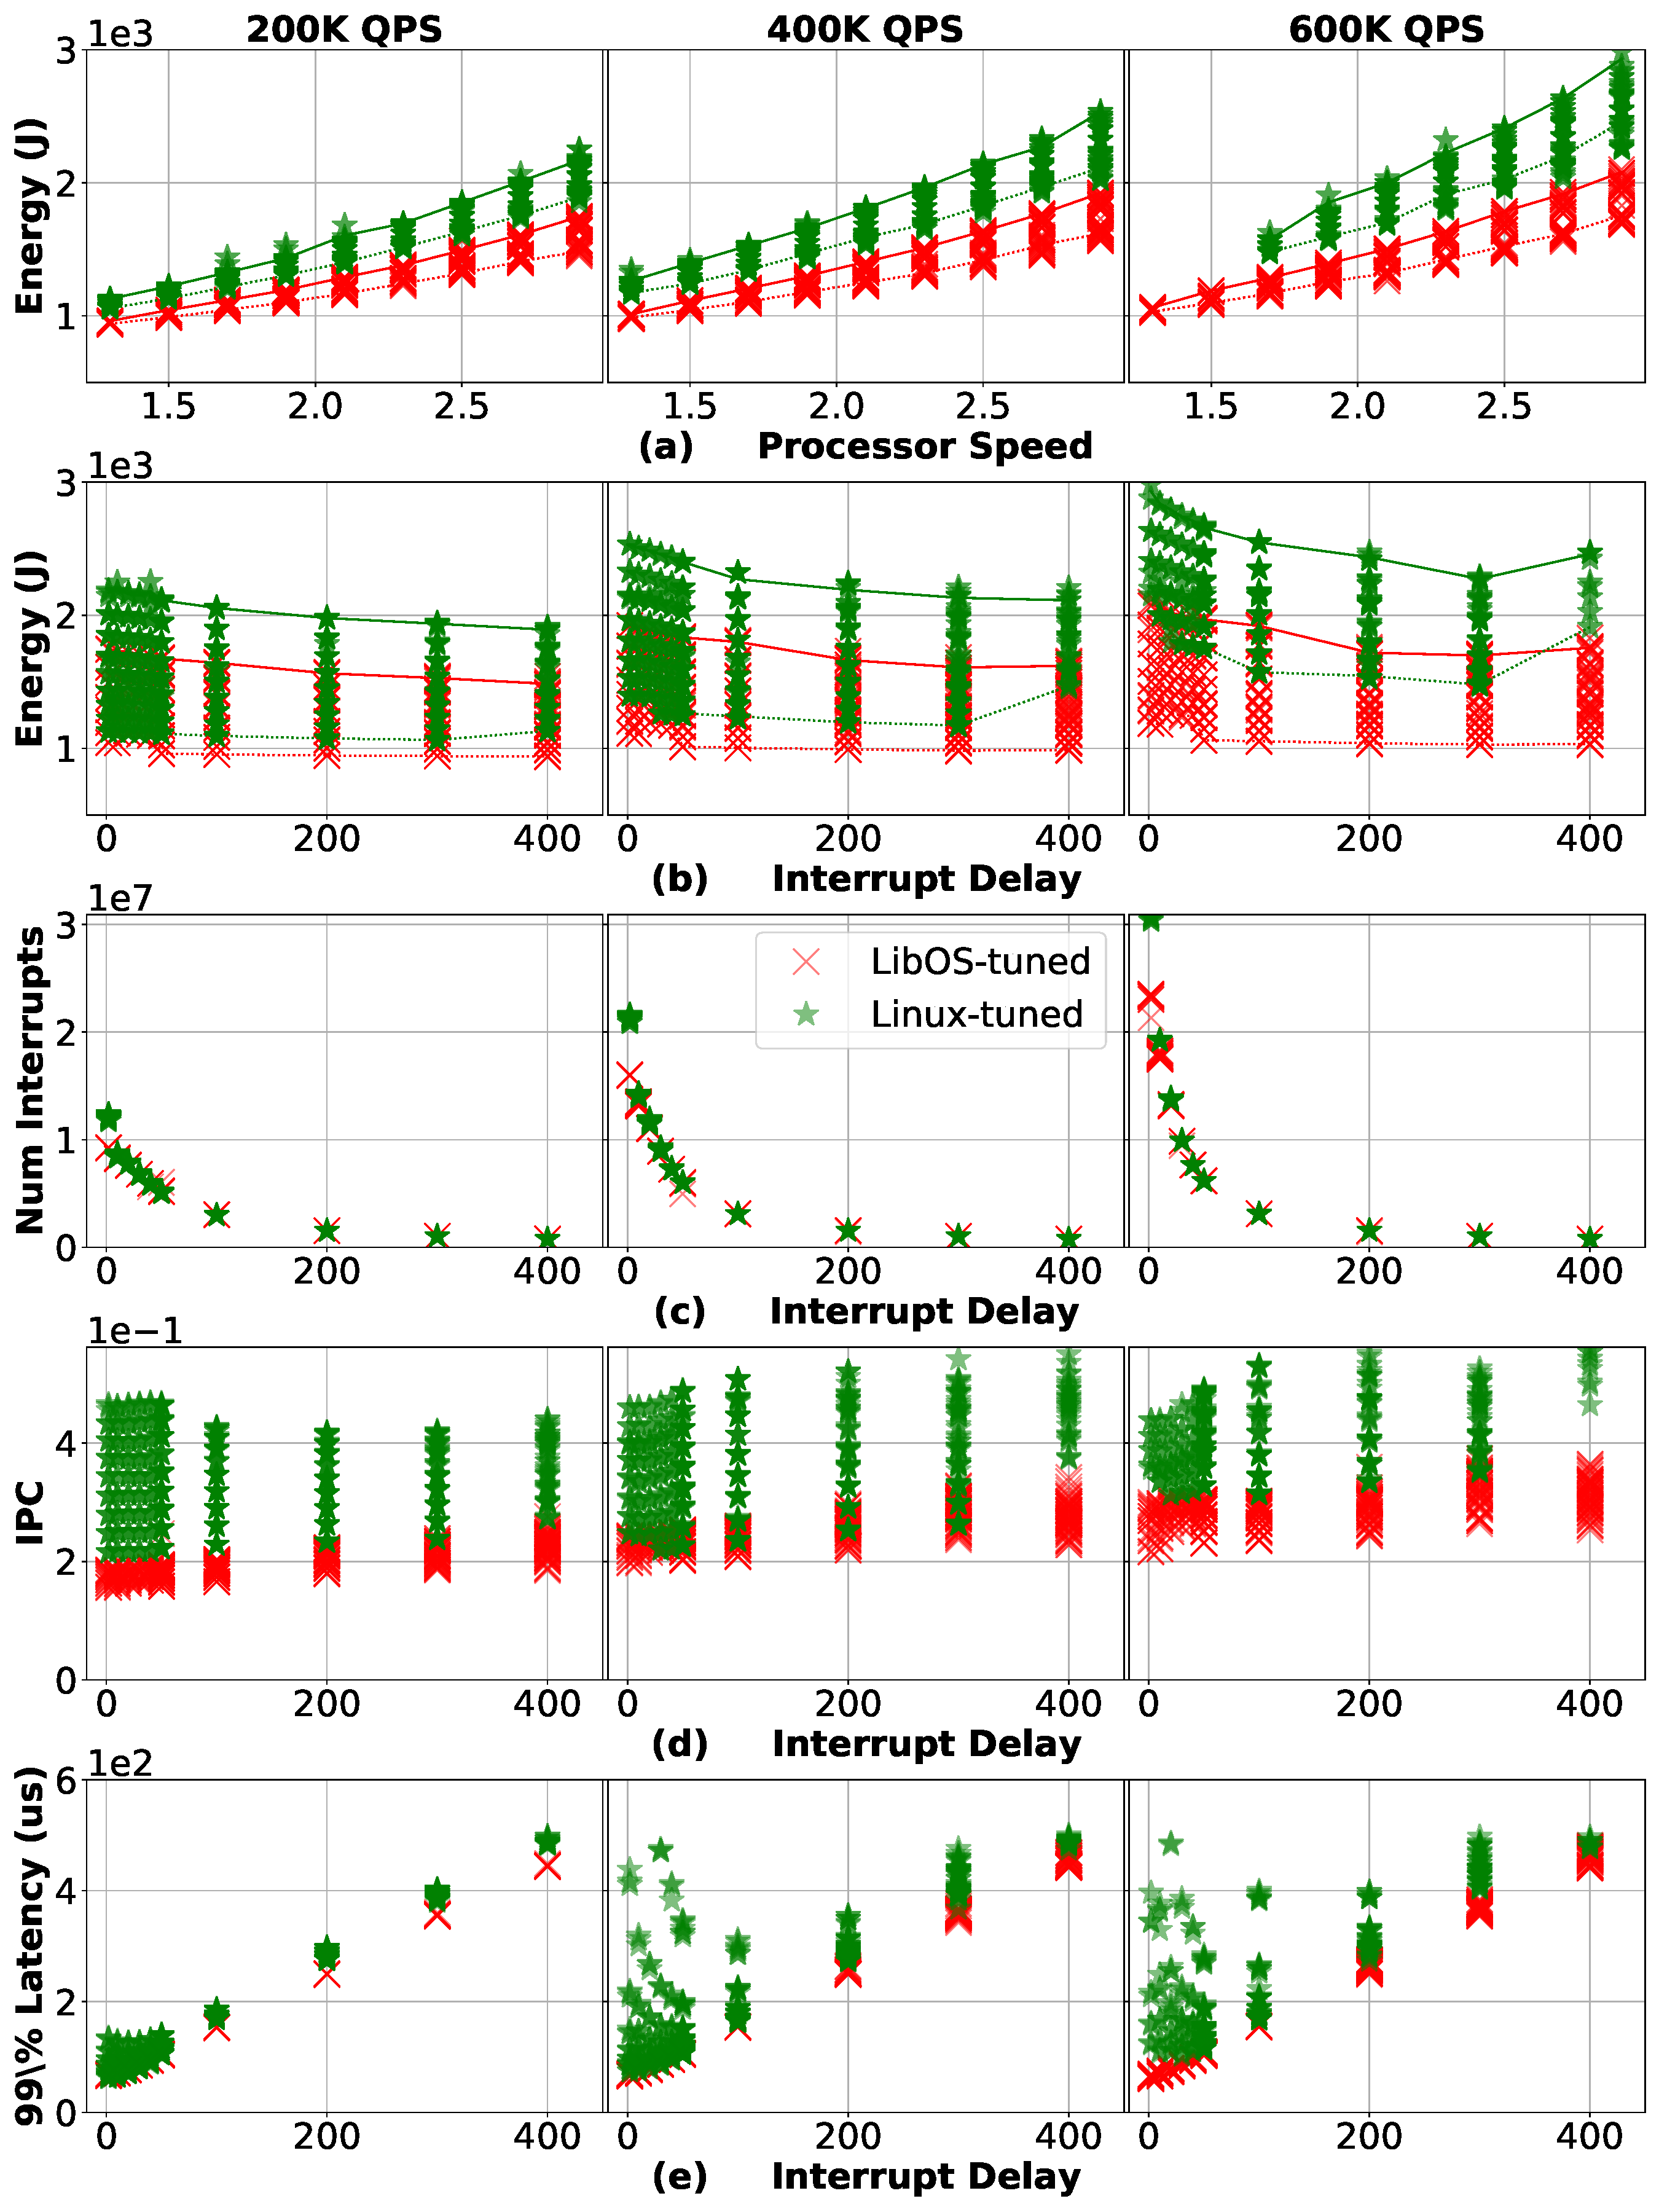
\includegraphics[width=0.5\textwidth]{figures/mcd_detail_1}
%\hspace*{-10.0cm} 
%\vspace*{-1.0cm}  
\caption[]{}
\label{fig:mcd_detail_1}
\end{figure}
\begin{figure}
%\centering
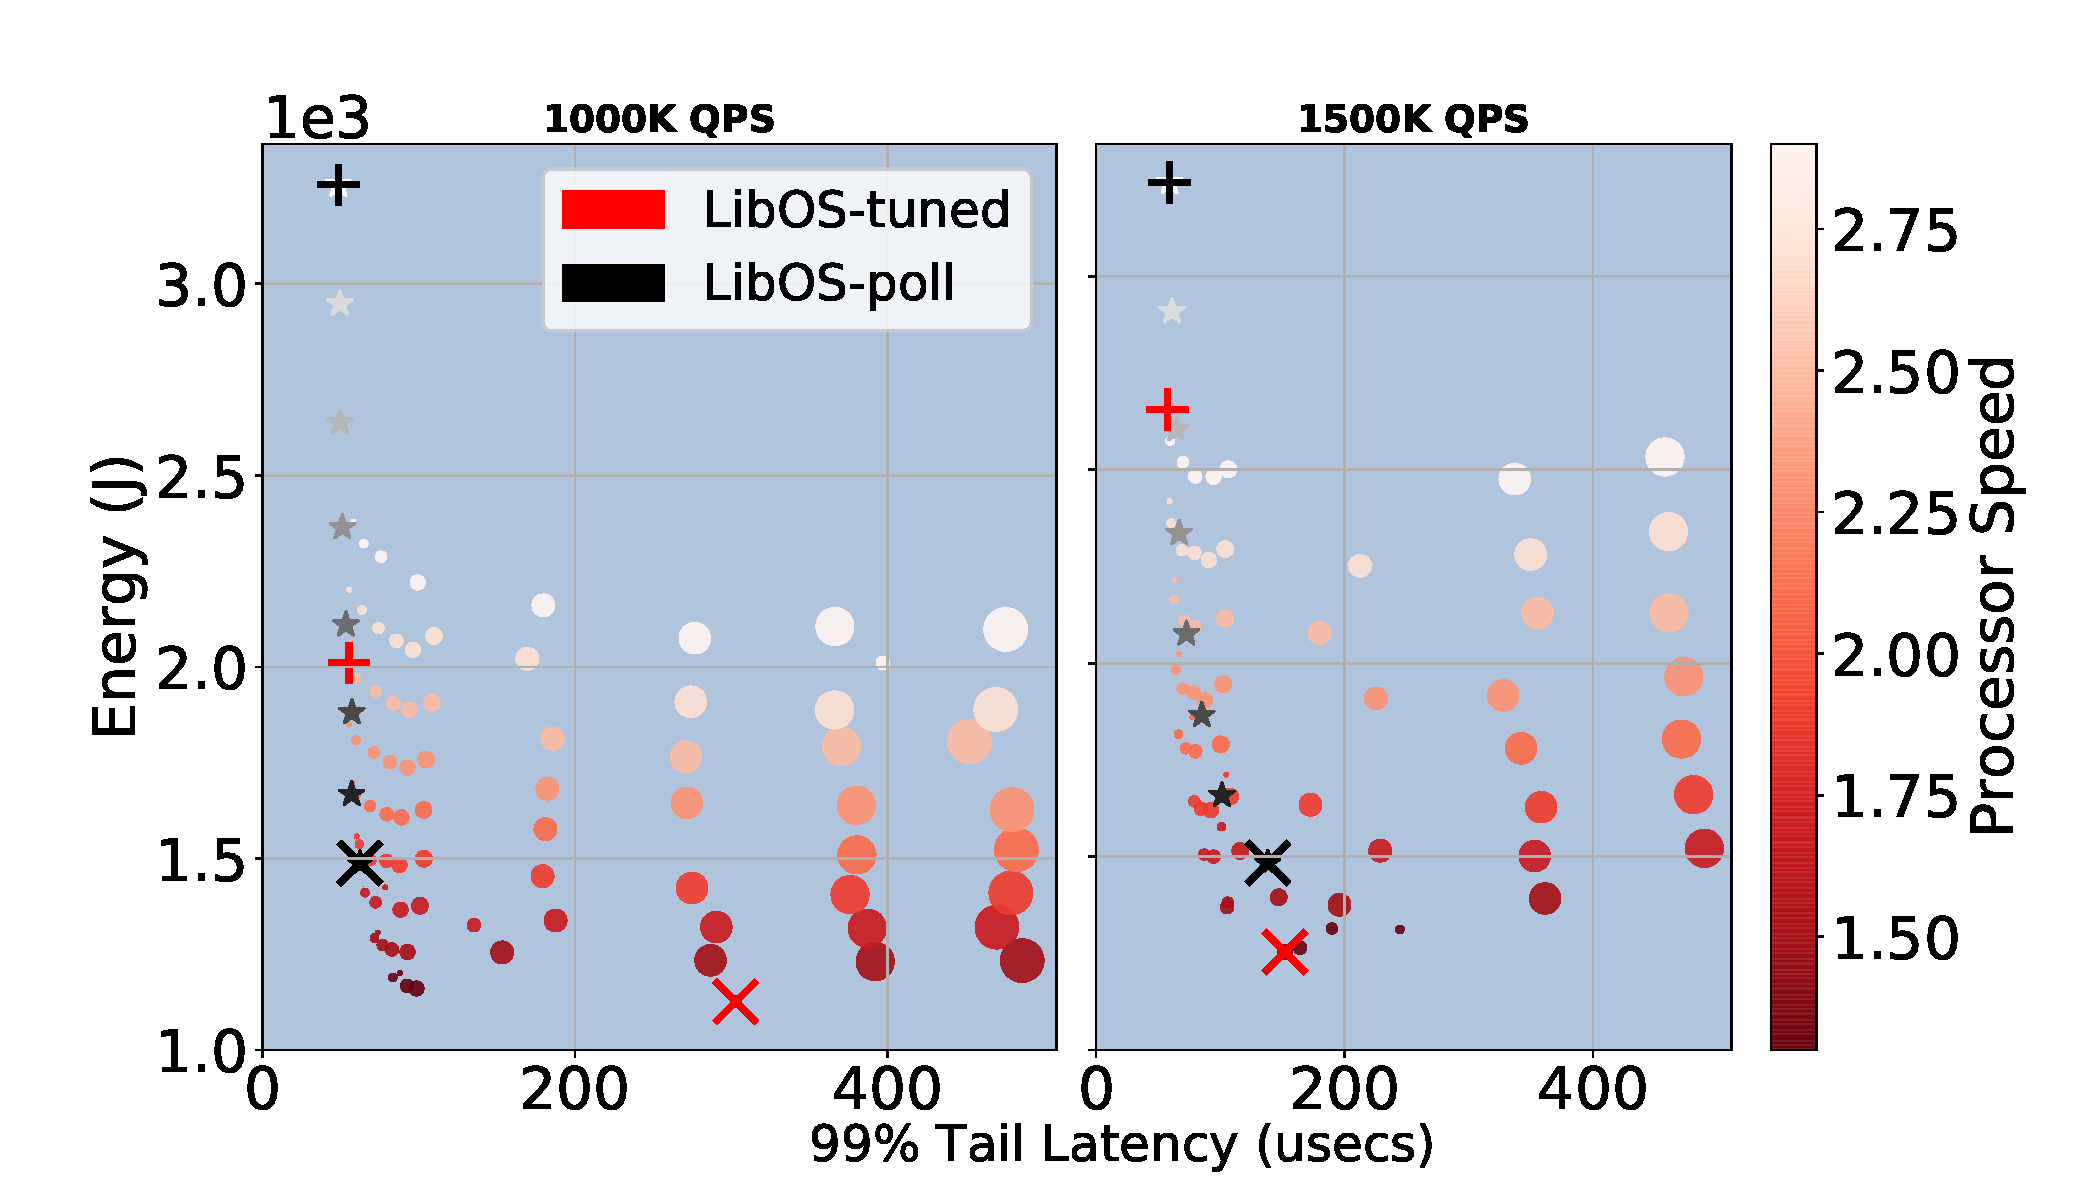
\includegraphics[width=0.5\textwidth]{figures/mcd_overview2}
%\vspace*{-1.0cm}  
\caption[]{}
\label{fig:mcd_overview2}
\end{figure}
% 200000 ebbrt_tuned 
%  	 SLOW-ITR-diff-Min-Max-DVFS= 702.25 J
%  	 FAST-ITR-diff-Min-Max-DVFS= 544.91 J

% 200000 linux_tuned 
%  	 SLOW-ITR-diff-Min-Max-DVFS= 1041.8 J
%  	 FAST-ITR-diff-Min-Max-DVFS= 760.76 J

% 400000 ebbrt_tuned 
%  	 SLOW-ITR-diff-Min-Max-DVFS= 809.36 J
%  	 FAST-ITR-diff-Min-Max-DVFS= 632.57 J

% 400000 linux_tuned 
%  	 SLOW-ITR-diff-Min-Max-DVFS= 1135.93 J
%  	 FAST-ITR-diff-Min-Max-DVFS= 644.14 J

% 600000 ebbrt_tuned 
%  	 SLOW-ITR-diff-Min-Max-DVFS= 891.97 J
%  	 FAST-ITR-diff-Min-Max-DVFS= 723.47 J

% 600000 linux_tuned 
%  	 SLOW-ITR-diff-Min-Max-DVFS= 706.79 J
%  	 FAST-ITR-diff-Min-Max-DVFS= 547.11 J
Memcached~\cite{mcd} is a multi-threaded open loop workload that runs on all 16 cores of any one of our server nodes. It consists of an unloaded client node running mutilate~\cite{mutilate}. This client (1) coordinates with five other mutilate agent nodes in order to generate requests to the server and (2) measures tail latency of all requests made. All five agent nodes are 16-core machines, whereby each core creates 16 connections, for a total of 1280 connections. This setup is able to saturate the single 16-core server\footnote{Mutilate is configured to pipeline up to four connections to further increase its request rate.}. Linux runs memcached-1.6.6 and our library OS uses a re-implemented version of memcached, written to the OS's interfaces, which supports the standard memcached binary protocol. To alleviate lock contention, an RCU hashtable is used to store key-value pairs. We run a representative load from Facebook~\cite{workloadanalysisfacebook} (ETC) which represents the highest capacity deployment. It uses 20 - 70 byte keys and 1 byte to 1 KB values and contains 75\% GET requests.

%\subsubsection{Slowing down processor has better performance-energy trade-offs for memcached than using sleep states.} 
%\label{sec:mcd:slowproctradeoff} 
%Figure~\ref{fig:mcd_detail_1}(b) shows that even though interrupts are slowed down, the energy differences within each interrupt delay is largely determined by the differences in processor speeds. The bold lines connect the mean energy use of each interrupt delay whereby processor speed is fastest while the dotted lines connect the mean energy use where processor speed is slowest. Compared to figure~\ref{fig:mcd_detail_1}(a), where the differences in energy use is caused by different interrupt delays, we find that reducing energy use by slowing down the \textit{processor} is 2-10X more effective than by slowing down \textit{interrupt delays} (i.e. increased potential for using sleep states) across different QPS rates and OS as well. We believe the main reason is that memcached workloads are bursty with multiple requests pipelined onto multiple cores, therefore the system as whole is always busy with work. This renders potential energy savings by prolonged periods of idleness not as effective as slowing down the processor itself. It should also be noted that Linux at 600K QPS has a smaller energy gap at an interrupt delay of \SI{400}{\micro s} due to the fact that SLA violations already started to occur at faster processor speeds.

% 200000 ebbrt_tuned 
%  	 SLOW-DVFS-diff-Min-Max-ITR= 21.11 J
%  	 FAST-DVFS-diff-Min-Max-ITR= 260.41 J
%  	 FAST/SLOW= 12.3359
% 200000 linux_tuned 
%  	 SLOW-DVFS-diff-Min-Max-ITR= 70.94 J
%  	 FAST-DVFS-diff-Min-Max-ITR= 277.91 J
%  	 FAST/SLOW= 3.9175
% 400000 ebbrt_tuned 
%  	 SLOW-DVFS-diff-Min-Max-ITR= 25.48 J
%  	 FAST-DVFS-diff-Min-Max-ITR= 302.86 J
%  	 FAST/SLOW= 11.8862
% 400000 linux_tuned 
%  	 SLOW-DVFS-diff-Min-Max-ITR= 90.47 J
%  	 FAST-DVFS-diff-Min-Max-ITR= 420.31 J
%  	 FAST/SLOW= 4.6458
% 600000 ebbrt_tuned 
%  	 SLOW-DVFS-diff-Min-Max-ITR= 30.19 J
%  	 FAST-DVFS-diff-Min-Max-ITR= 325.17 J
%  	 FAST/SLOW= 10.7708
% 600000 linux_tuned 
%  	 SLOW-DVFS-diff-Min-Max-ITR= 92.84 J
%  	 FAST-DVFS-diff-Min-Max-ITR= 471.21 J
%  	 FAST/SLOW= 5.0755
\subsubsection{Slowing down processor diminishes energy savings of using sleep states}
\label{sec:mcd:slowprocvssleep}
Figure~\ref{fig:mcd_detail_1}(a) shows that as a processor slows down, the energy savings from slow downing down interrupts also decreases (larger energy gap to smaller energy gap). Bold lines indicate the mean energy use at fastest interrupt delay, while dotted lines indicate mean energy use at slowest. We find that across the QPS loads and the two OSes, the average energy savings from slowing down interrupt delay at the \textit{slowest} processor speed is an average of \SI{52}{\joule} while at the \textit{fastest} processor speed we get a average energy savings of \SI{342}{\joule}. Detailed in section~\ref{sec:workflow:dvfs}, the effect of slowing down the processor results in the lengthening of the application and OS work in memcached, thereby reducing the benefits of prolonged idle periods to take advantage of energy savings by sleep states, this is also further exacerbated by the SLA requirements which results in a strict time budget each request must adhere to. 

Even though slowing down interrupt delay does not contribute to energy savings as much as slowing down the processor, figure~\ref{fig:mcd_overview} shows that it is  with a combination of both that results in the lowest energy use across both Linux and libOS. Figure~\ref{fig:mcd_detail_1}(e) shows the direct effect of interrupt delay on tail latency; the benefit of slowing down interrupt rates consists of 1) lowering the number of interrupts fired, which also lowers instruction use and potentially promotes better packet coalescing (see figures~\ref{fig:mcd_detail_1}(c)(d)), and 2) based off interrupt delay algorithm in figure~\ref{fig:itr_delay_flowchart} and detailed in section~\ref{sec:workflow:itrdelay}, this ensures a guaranteed period of quiescence such that the processor can take advantage of potentially deeper sleep states. However, we hypothesize these trade-offs will be different dependent on other factors such as an OS's packet processing efficiency and policies that govern the use of sleep states to maximize quiescence states. Moreover, the benefit of slowing down interrupt rates versus processor is a more subtle debate as the implications of slowing down the processor affects all software whereas interrupt delay is a fixed rate that will always wake up the software (if there is work) at some point in the future to handle the interrupt. Manually controlling the interrupt delay value also interacts with sleep state policies in terms of processor wakeup time, sleep state selection, and potential energy-performance trade-offs within this space. 
%Embedded inside the interrupt delay value a
%is an entirely hardware construct outside the purview of software other than knowing at some fixed point in the future to waking up to handle the interrupt.
% Based off these observations, one can assert that to optimize energy savings at a cost to tail latency for memcached involves slowing down both processor and interrupt rate,
%Second, we find that in the libOS, slowing down interrupt rates at the fastest processor speed results in around 11X better energy savings over the slowest processor speed. Similarly we find the same benefits in Linux, however, the energy savings are only around 4X better.
\subsubsection{Slowing down in different OS structures } 
\label{sec:mcd:slowinos}
%Even though figure~\ref{fig:mcd_overview} indicates the libOS uses lower energy than Linux across all QPS loads, we find that in both figures~\ref{fig:mcd_detail_1}(a)(b), Linux is always able to save more energy (1.02X to 3.6X) by slowing down processor and interrupt rates than the libOS. We believe this more a result of the base efficiency of libOS' 
The \textit{vertical-ness} of the library OS points in figure~\ref{fig:mcd_overview} largely shows the ineffectiveness of slowing down the processor in causing a increase in the tail latency; we attribute this to the efficiency of the memcached implementation in the library OS system as a whole. As discussed in section~\ref{sec:workflow:dvfs}, we found that although LibOS-tuned has worse IPC than Linux-tuned across the QPS loads (figure~\ref{fig:mcd_detail_1}(d)), it also used on average ~2.5X fewer instructions than Linux. Furthermore, figure~\ref{fig:mcd_overview2} demonstrate that the library OS can support higher QPS loads than Linux. We can see the opposite of this behavior in Linux where at 600K QPS, it is approach 75\% of the peak QPS it can support, there is a clear trade-off between slowing down processor speeds and an increase in tail latency (higher latency points tend to have darker gradient color). In figure~\ref{fig:mcd_overview2}, memcached is scaled higher to 1500K QPS load, which is around 75\% of the library OS' peak it can support, at this QPS rate we can begin to see similar trade-offs as Linux.

% MIN-TAIL linux_default 200000 1 3.0 135    103.3 1335.43
% MIN-TAIL linux_tuned 200000 2 2.9 135       61.7 2174.6

% MIN-TAIL linux_default 400000 1 3.0 135    111.9 1927.74
% MIN-TAIL linux_tuned 400000 2 2.9 135       74.0 2532.51

% MIN-TAIL linux_default 600000 1 3.0 135    137.5 2594.01
% MIN-TAIL linux_tuned 600000 30 2.9 135     102.6 2730.61

% Linux's network driver contains a interrupt moderation algorithm is a generic algorithm used to cater the interrupt delay rate towards the current traffic pattern to maximize throughput.
\subsubsection{Fast interrupt rates induces low tail latency at high energy use.} 
\label{sec:mcd:fastitr} 
Figure~\ref{fig:mcd_overview} also demonstrates the ability to use a fast interrupt delay in order to minimize tail latency. Linux-tuned improved its tail latency over Linux-default by 40\% at 200K QPS and 25\% at 600K QPS. As discussed in section~\ref{sec:workflow:hybridio}, a faster interrupt delay can induce a form of polling with Linux's NAPI policy by constantly waking up the processor to do the OS and application work. This induced behavior also increases energy use by 38\% at 200K QPS and 5\% at 600K QPS; which represents another space in the energy-performance trade-off of memcached. While some prior research have used statically setting the interrupt delay rate at a low value for experimental stability~\cite{10.1145/2812806, 10.5555/3323234.3323265}, we are the first to show its energy implications.

% MIN-TAIL ebbrt_tuned 200000 2 0x1d00 135        65.9 1747.17
% MIN-ENERGY ebbrt_tuned 200000 400 0xd00 55     444.3  935.44  
% MIN-TAIL ebbrt_tuned 1500000 50 0x1500 135     100.4 1790.14
% MIN-ENERGY ebbrt_tuned 1500000 100 0xf00 135   195.9 1375.67 

% ebbrt_tuned c1 200000 2 0x1d00 135 47.1 1910.13 13115025 9645754
% ebbrt_tuned c1e 200000 2 0x1d00 135 67.4 1772.53 10777190 9203709
% ebbrt_tuned c3 200000 2 0x1d00 135 67.7 1780.14 10747417 9196942
% ebbrt_tuned c7 200000 2 0x1d00 135 68.1 1774.63 10827352 9218834

% ebbrt_tuned c1 200000 400 0xd00 135 442.8 948.19 3291640 781241
% ebbrt_tuned c1e 200000 400 0xd00 135 445.1 941.39 2950100 781239
% ebbrt_tuned c3 200000 400 0xd00 135 445.1 935.63 2676159 781228
% ebbrt_tuned c7 200000 400 0xd00 135 443.8 943.83 3594352 781236

% ebbrt_tuned c1 1500000 0 0x1d00 135 58.5 2633.76 33730121 318342
% ebbrt_tuned c1e 1500000 0 0x1d00 135 59.3 2614.47 31964816 318347
% ebbrt_tuned c3 1500000 0 0x1d00 135 58.9 2640.36 31464117 318348
% ebbrt_tuned c7 1500000 0 0x1d00 135 57.7 2631.38 31876151 318346

% ebbrt_tuned c1 1500000 100 0xf00 135 171.1 1343.02 3939748 312496
% ebbrt_tuned c1e 1500000 100 0xf00 135 191.3 1343.54 3557152 312496
% ebbrt_tuned c3 1500000 100 0xf00 135 196.1 1336.57 3599566 312488
% ebbrt_tuned c7 1500000 100 0xf00 135 195.9 1375.84 3558380 312495
% \begin{table}[t]
% \centering
% \begin{tabular}{l|c|c|c|c|c|}
%   QPS & Type & Sleep State & Latency (\SI{}{\micro s}) & Energy (\SI{}{\joule})\\ \hline
%   200K & Min-Tail & C1 & 47 & 1910\\ \hline
%   200K & Min-Tail & C1E & 57 & 1772\\ \hline
%   200K & Min-Tail & C3 & 67 & 1770\\ \hline
%   200K & Min-Tail & C7 & 68 & 1774\\ \hline
%   200K & Min-Energy & C1 & 442 & 949\\ \hline
%   200K & Min-Energy & C1E & 445 & 941\\ \hline
%   200K & Min-Energy & C3 & 445 & 941\\ \hline
%   200K & Min-Energy & C7 & 443 & 937\\ \hline
%   1500K & Min-Tail & C1 & 58 & 2633\\ \hline
%   1500K & Min-Tail & C1E & 59 & 2614\\ \hline
%   1500K & Min-Tail & C3 & 59 & 2640\\ \hline
%   1500K & Min-Tail & C7 & 58 & 2631\\ \hline
%   1500K & Min-Energy & C1 & 171 & 1343 \\ \hline
%   1500K & Min-Energy & C1E & 191 & 1343\\ \hline
%   1500K & Min-Energy & C3 & 196 & 1336\\ \hline
%   1500K & Min-Energy & C7 & 195 & 1375\\ \hline
% \end{tabular}
% \caption{Min-Tail refers to configuration of processor speed and interrupt rate where the lowest tail latency was achieved and Min-Energy refers to the configuration with lowest energy use.}
% %\caption{Workload configurations.
% %The column {\em Nature} indicates open-versus-closed loop nature
% %and {\em CPU} indicates application CPU demand.}
% \label{table:mcd_sleep_states}	
% \end{table}

% \subsubsection{Finding-5: Sleep states and race-to-halt rarely useful)} \label{sec:f5} 
% Table~\ref{table:mcd_sleep_states} lists a small experiment where different sleep states are explored under the libOS at two extremities when the libOS is lightly loaded (200K QPS) and heavily loaded (1500K QPS). \textit{Min-Tail} is configuring the processor and interrupt rate running fastest while \textit{Min-Energy} is both parameters running slowest. When the libOS is lightly loaded, we find that using different sleep states does make a difference in tail latency and energy. We hypothesize that the small exit latencies of the C1 sleep state results in better tail latencies for memcached. However, we find the effect is lessened when under a heavier load, which seems to indicate that a slowed processor is affecting the efficacy of sleep states given it is already running at a slowed interrupt delay rate, which implies ample opportunities to take advantage of system idling. Moreover, as the load increases for the libOS, selection of different sleep states causes no noticeable differences in either latency nor energy, which implies the constant bursty nature of incoming packets is rendering the idle times non-existent. Lastly, combined with the energy benefits of slowing down the processor versus using sleep states in ~\ref{sec:f2}, we assert that trying to use sleep states for energy savings is largely ineffective. 

\subsubsection{Polling can be energy efficient}
\label{sec:mcd:poll}
Similar to netpipe 64B (figure~\ref{fig:closed_loop_overview}), figure~\ref{fig:mcd_overview} shows that using an OS poll for network workloads with a small payload results in the best performance (tail latency) in memcached. Although memcached is a more complex workload with thousands of connections and requests pipelined and multiplexed on multiple cores, LibOS-poll is can still be energy efficient through slowing down the processor. Using \textbf{X} point (Min-Energy) of LibOS-poll as reference, we find that at 200K QPS, LibOS-poll improves both the tail latency and energy over LibOS-tuned at \textbf{+} (Min-Latency) by 20\%. As the load increases, by comparing the Min-Energy points, we find that while LibOS-poll consumes 11\%-38\% more energy across all QPSes, its tail latency was 10\%-90\% better. Our experiment with slowing down processor in a library OS poll reveals an additional trade-off space for energy-performance in memcached.


% MIN-TAIL ebbrt_tuned   200000 2 0x1d00 135    65.9 1747.17
% MIN-TAIL ebbrt_poll    200000 666 0x1d00 135  44.3 3239.33
% MIN-ENERGY ebbrt_tuned 200000 400 0xd00 55   444.3 935.44 = 415615
% MIN-ENERGY ebbrt_poll  200000 666 0xd00 135   52.4 1296.02 = 67910

% MIN-TAIL ebbrt_tuned   400000 2 0xf00 55      64.9 1111.27
% MIN-TAIL ebbrt_poll    400000 666 0x1b00 135  45.1 2900.71
% MIN-ENERGY ebbrt_tuned 400000 300 0xd00 55   366.6 976.33 
% MIN-ENERGY ebbrt_poll  400000 666 0xd00 135   59.2 1299.53 

% MIN-TAIL ebbrt_tuned   600000 2 0x1100 55     60.2 1278.68
% MIN-TAIL ebbrt_poll    600000 666 0x1d00 135  46.0 3242.68
% MIN-ENERGY ebbrt_tuned 600000 400 0xd00 55   482.0 1025.02 
% MIN-ENERGY ebbrt_poll  600000 666 0xd00 135   61.5 1295.59 

% MIN-TAIL ebbrt_tuned   1000000 2 0x1900 135     55.3 2010.23
% MIN-TAIL ebbrt_poll    1000000 666 0x1d00 135   48.6 3258.35
% MIN-ENERGY ebbrt_tuned 1000000 20 0xd00 135    303.0 1126.13 
% MIN-ENERGY ebbrt_poll  1000000 666 0xf00 135    62.4 1487.28 

% MIN-TAIL ebbrt_tuned   1500000 2 0x1d00 135     57.4 2655.69
% MIN-TAIL ebbrt_poll    1500000 666 0x1d00 135   59.1 3242.74
% MIN-ENERGY ebbrt_tuned 1500000 40 0xd00 135    152.0 1253.26 
% MIN-ENERGY ebbrt_poll  1500000 666 0xf00 135   138.2 1483.45 





%\textbf{Polling - TODO}
%how is it done
%shortened os path length keep it busy during idle periods makes energy lat tradeoff competitive
